\documentclass{beamer}
\usepackage[utf8]{inputenc}
\usepackage{pre}
\usetheme{Madrid}
\usecolortheme{default}
\setbeamertemplate{bibliography item}[text]
\bibliographystyle{plain}

\title[Final project] 
{Group Final project: Preparation}

% \author{Lin Yuheng}
\author{8-Hengke Jiang, 11-Rock, 13-Yuting Jiang, 30-Ethan, 35-Jade Lin}

\institute[] % (optional)
{ 
  {linyh63@mail2.sysu.edu.cn}
}

\date[6.30.2024] % (optional)
% {Agust 25, 2023}

\AtBeginSection[]
{
  \begin{frame}
    \frametitle{Table of Contents}
    \tableofcontents[currentsection]
  \end{frame}
}

\begin{document}
\frame{\titlepage}
% \tableofcontents
\section{Introduction}
\begin{frame}
  \frametitle{Natural Language Processing(NLP)}
  
  \begin{figure}[H]
    \centering
    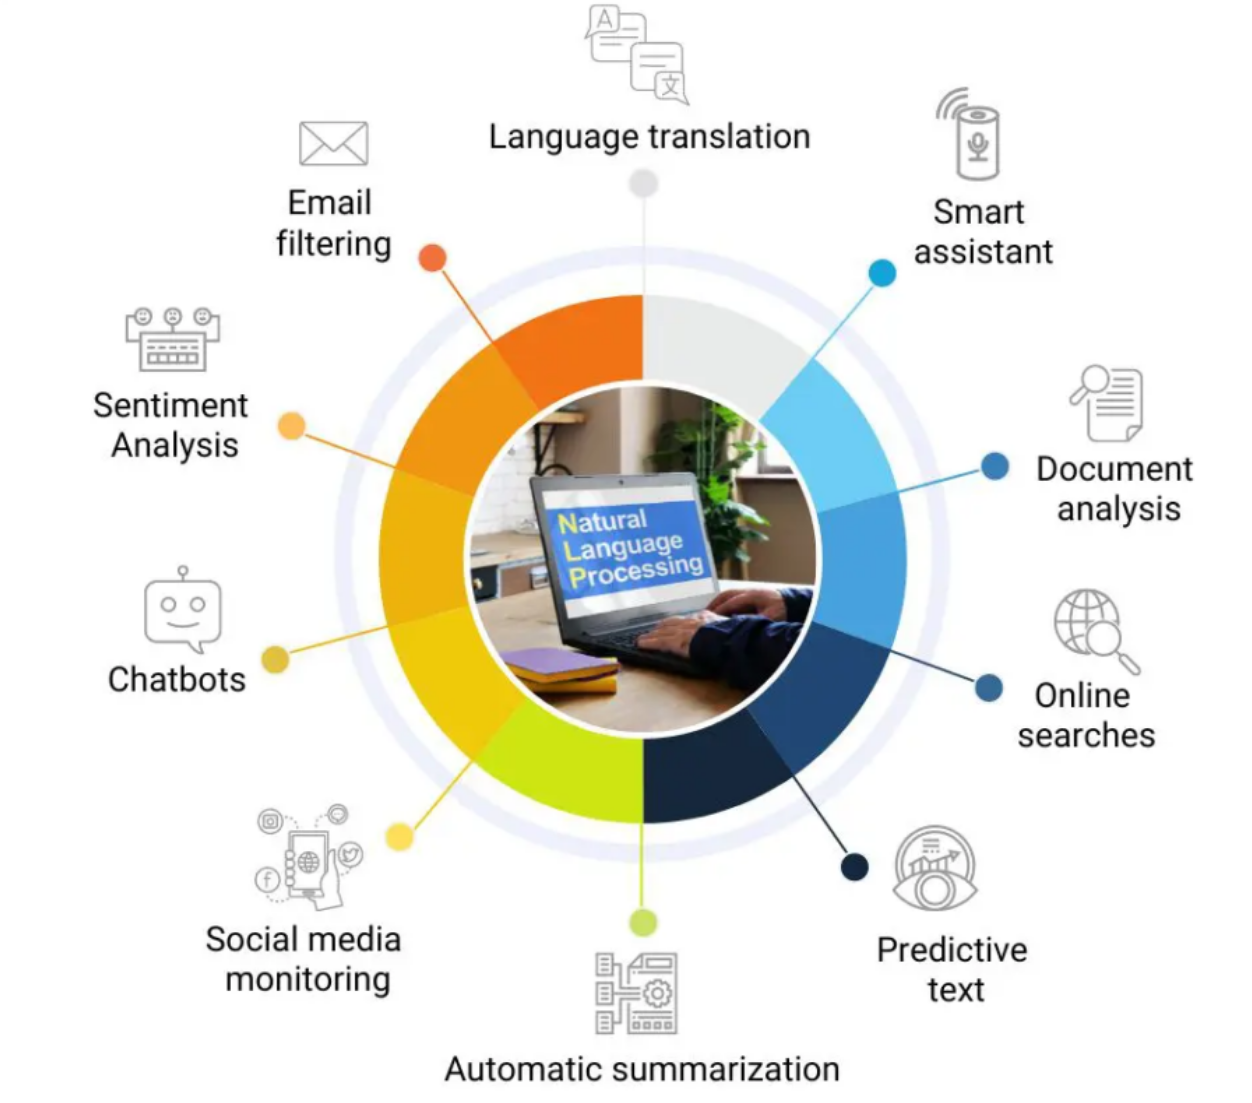
\includegraphics[width=8cm]{D:/Pictures/Screenshots/屏幕截图 2024-06-30 163118.png}
  \end{figure}
\end{frame}
\begin{frame}
  \frametitle{History}
  Before the invention of computer, Alan Turing published an article titled "Computing Machinery and Intelligence" which proposed what is now called the Turing test as a criterion of intelligence.(1940)\\\

  With computer, machine translation(MT) and Statistical machine translation(SMT).(1950-1900, 1990-2010)\\\

  Multi-layer perceptron(MLP, 2003), recurrent neural network(RNN, 2010)...
\end{frame}
\section{Modern NLP and SOA}
\begin{frame}
  \frametitle{Attention is all you need}
  \begin{figure}[H]
    \centering
    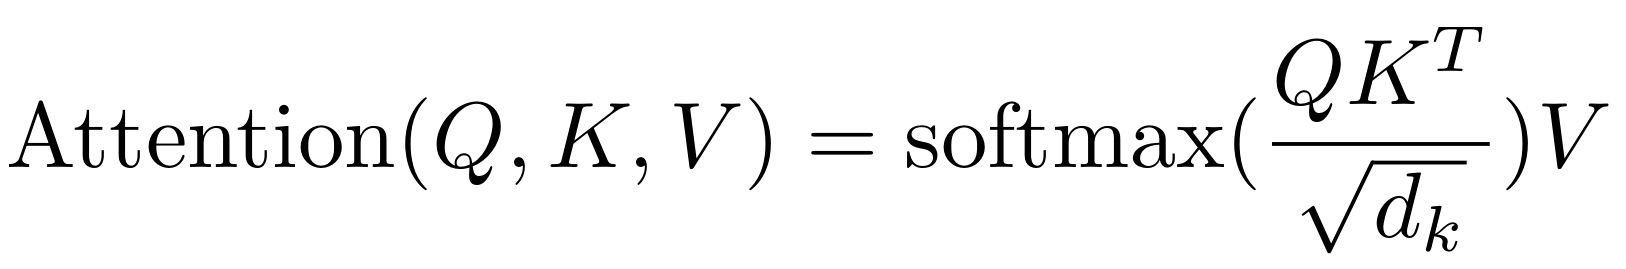
\includegraphics[width=8cm]{D:/Pictures/Screenshots/屏幕截图 2024-06-30 171741.png}
  \end{figure}
  Transformers use self-attention mechanisms to process input sequences in parallel, making them highly efficient and effective.(6.2017\cite{vaswani2023attentionneed})\\\
  \begin{figure}[H]
    \centering
    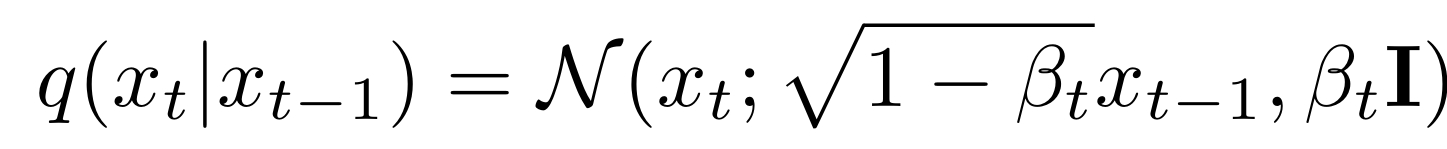
\includegraphics[width=8cm]{D:/Pictures/Screenshots/屏幕截图 2024-06-30 171707.png}
  \end{figure}

  Base on Denoising Diffusion Probabilistic Models(2020, DDPM\cite{ho2020denoisingdiffusionprobabilisticmodels})
  diffusion(2021, \cite{austin2023structureddenoisingdiffusionmodels}) and continuous diffusions(2022, Diffusion-LM\cite{li2022diffusionlmimprovescontrollabletext}) are introduced to improve non-autoregressive(NAR) text generation.

\end{frame}
% \begin{frame}
%   %\frametitle{}
%   \begin{figure}[H]
%     \centering
%     \includegraphics[width=10cm]{D:/Pictures/Screenshots/}
%     % \caption{}
%   \end{figure}
% \end{frame}
\begin{frame}{Bibliography}
  \bibliography{cite.bib}
\end{frame}
\end{document}